
To validate the applicability of our method we have developed a case study concerning risk assessment for financial companies as implemented by the ORCA System\footnote{The ORCA System is a trademark of GCP Global (www.gcpglobal.com).}.
Risk assessment is implemented by an interactive business process based on the exchange of a series of questionnaires intended to evaluate the risks implied by the client business practice.
Examples of business practices are: the conditions and protocols used to perform confidential transactions, the physical security to access reserved areas (such as computing server installations).
The information gathered by the questionnaires is used to evaluate whether there are risky practices within the business processes of the company, as well as to propose amendments to these practices.
The ultimate goal of the risk assessment is to determine a degree of compliance to existing standards.
By analyzing the questionnaires, ORCA detects risky practices, proposes solutions and triggers further assessment processes to ensure that the solutions have been implemented.

Our goal is to model a service based application (\FlyingPig), for providing risk assessment as a service.
In order to provide this functionality, \FlyingPig\ benefits from ORCA's legacy services providing storage, assessment and data visualization functions.

In the following sections, we describe the results of applying \pisodm to develop the \FlyingPig\ risk assessment system.
The models presented next were generated as a result of interacting with software developers at GCP Global.

\begin{figure*}
\centering
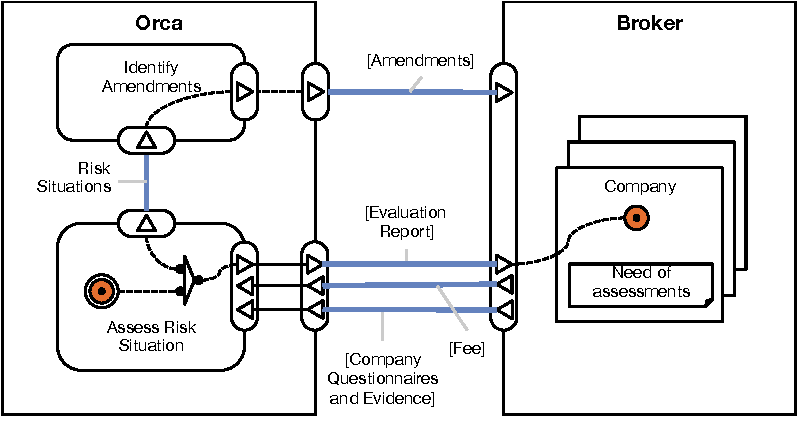
\includegraphics[width=0.9\textwidth]{figs/3ValueModel.pdf}
\hspace*{5cm}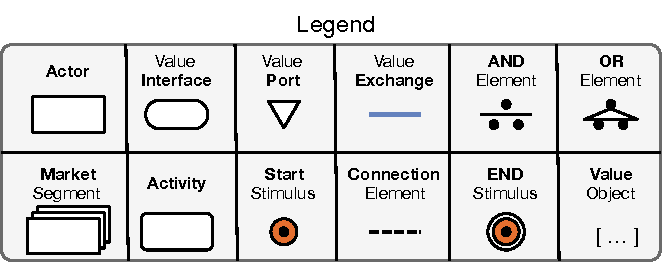
\includegraphics[width=0.4\textwidth]{figs/3ValueKey.pdf}
\caption{E3value model for \FlyingPig.\label{fig:E3valuemodel}}
\end{figure*}

%. . - -. . - -. . - -. . - -. . - -. . - -. . - -. . - -. . - -. . - -. . - -. . - -. . - -. . - -. . - -. . - -. . - -. . - -. . - -. . - -. . - -. . - -. . - -. . - -. . - -. . - -
\subsection{Computation-Independent Models (CIM)}
%. . - -. . - -. . - -. . - -. . - -. . - -. . - -. . - -. . - -. . - -. . - -. . - -. . - -. . - -. . - -. . - -. . - -. . - -. . - -. . - -. . - -. . - -. . - -. . - -. . - -. . - -

Figure~\ref{fig:E3valuemodel} shows the value model for the \FlyingPig\ application.
It is a business model that graphically represents a business case as a set of value exchanges ($\triangleright$ and $\triangleleft$) and value activities (rounded boxes) performed by business actors (squared boxes).
%\footnote{\color{red} This sentence need to move to section 3.1!!}
We identify two business actors: \textsl{ORCA} and \textsl{Broker}.
Brokers emit requests for risk assessment for one or more companies.
ORCA has two value activities which are services that provide an economical benefit:  \textsl{Identify Amendments} and \textsl{Assess Risk Situation}.
The values exchanged between ORCA and the brokers are:
(i) \textsl{Questionnaire and Evidences} filled with information about the client company;
(ii) \textsl{Amendments} which are ORCA's rec\-om\-men\-da\-tions, based on the data provided by the answers to questionnaires;
(iii) \textsl{Evaluation Reports} for the client companies;
and
(iv) the risk assessment \textsl{fee}.

The dependency path in Figure~\ref{fig:E3valuemodel} initiates with the need of assessment emitted by a particular company.
Once this need has been declared, the value exchanges between ORCA and Broker are triggered.
The client company provides ORCA with information (answers to a questionnaire), evidence (to support the information) and a fee (monetary value).
In the next step, ORCA suggests amendments (recommendations to change practices) and provides an evaluation report.

\begin{figure*}
\centering
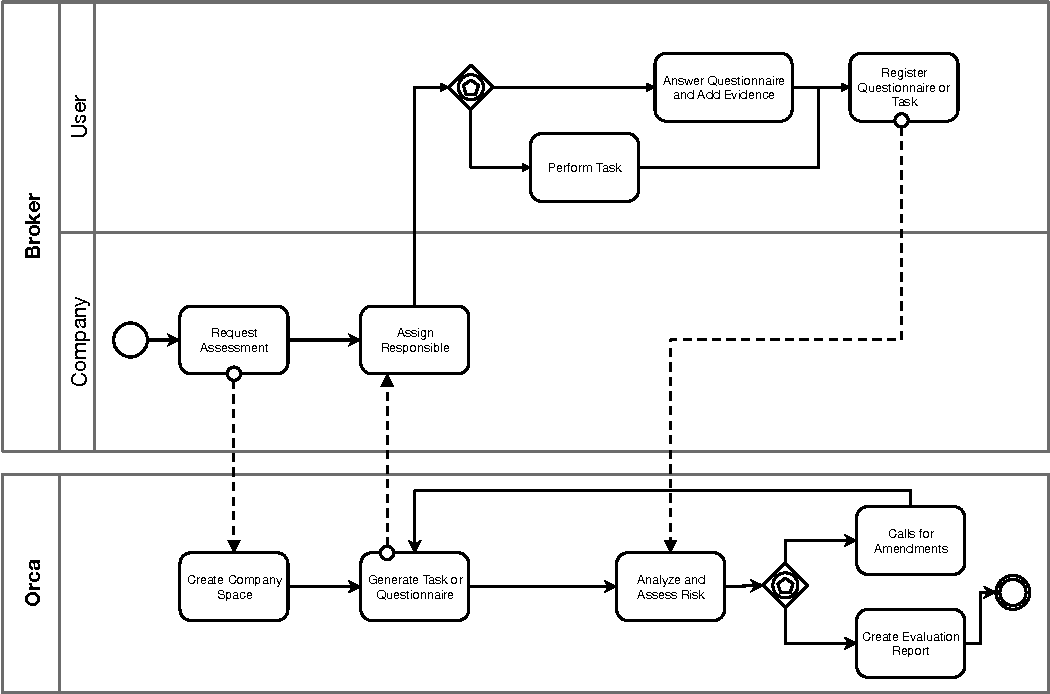
\includegraphics[width=1.0\textwidth]{figs/BPMN_GCP.pdf}
\caption{BPMN model for \FlyingPig.\label{fig:BPMNmodel}}
\end{figure*}


Figure~\ref{fig:BPMNmodel} shows the BPMN model
%\footnote{\color{red} Details on BPMN (Business Process Management Notation) can be found in http://www.bpmn.org/.}
for the \FlyingPig\ scenario. The BPMN model for \FlyingPig\ is partitioned for better understanding the process in which the value exchanges occur.
The model includes two pools representing the \textsl{ORCA} system and the \textsl{Brokers}.
Brokers have two lanes, the client \textsl{Company} and a \textsl{User}.
The user is a contact member of the company, who  coordinates the assessment process.
This process  involves other members of the company as well.

The risk assessment process starts after a request from a company.
This corresponds to the value model, in which the start stimulus triggers the whole process.
The request leads to the definition of a group of users that will answer questionnaires to evaluate risk.
Other tasks include amending a ``risky situation'' as well as producing evidence to show that a specific risk has been eliminated\footnote{Risky situations include  material facts such as not facilitating access to physically disabled people in a bank agency or having an unsecured access to the premises of the company.
They can be also abstract  such as the protocol used for accessing data on the company's computer server.}.

Once tasks have been completed, they are stored and analyzed to generate a list of non-compliant situations, associated to their corresponding \textit{calls for amendment} (if needed) or a report specifying a compliance level, incidents and a risk map.
During the process of analyzing a questionnaire, the answers to some questions may trigger the generation of additional questionnaires or amendments, that will be scheduled as new tasks.

Business processes also have rules and constraints to define their non-functional requirements (NFR):
\begin{numtrivlist}
\item An acknowledgement is due in less than 30 seconds after registering a task or demand for assessment.
\item The system should be able to deal with, at least, 200 users.
\item If the number of requests exceeds 200, \FlyingPig\ should implement a load balance strategy for processing the requests.
\item The privileges of the Channel-Broker must be verified \textit{before} the execution of the actions associated to the \textsf{designate user in charge} $\pi$-use case.
\item The privileges of users must be verified \textit{before} the execution of the actions associated to the \textsf{answer questionnaire and add evidences} $\pi$-use case.
\item All questionnaires need to be fully answered in order to consider that a task is completed.
\item There is a time limit (in days) for amendments required by the system.
\end{numtrivlist}



%. . - -. . - -. . - -. . - -. . - -. . - -. . - -. . - -. . - -. . - -. . - -. . - -. . - -. . - -. . - -. . - -. . - -. . - -. . - -. . - -. . - -. . - -. . - -. . - -. . - -. . - -
\subsection{Platform-Independent Models (PIM)}
%. . - -. . - -. . - -. . - -. . - -. . - -. . - -. . - -. . - -. . - -. . - -. . - -. . - -. . - -. . - -. . - -. . - -. . - -. . - -. . - -. . - -. . - -. . - -. . - -. . - -. . - -

%In Section~\ref{sec:modelingWithPISODM} we defined three models at the PIM level.
The \pisodm models of the PIM level  for the \FlyingPig\ scenario are presented next.

\begin{figure*}
\centering
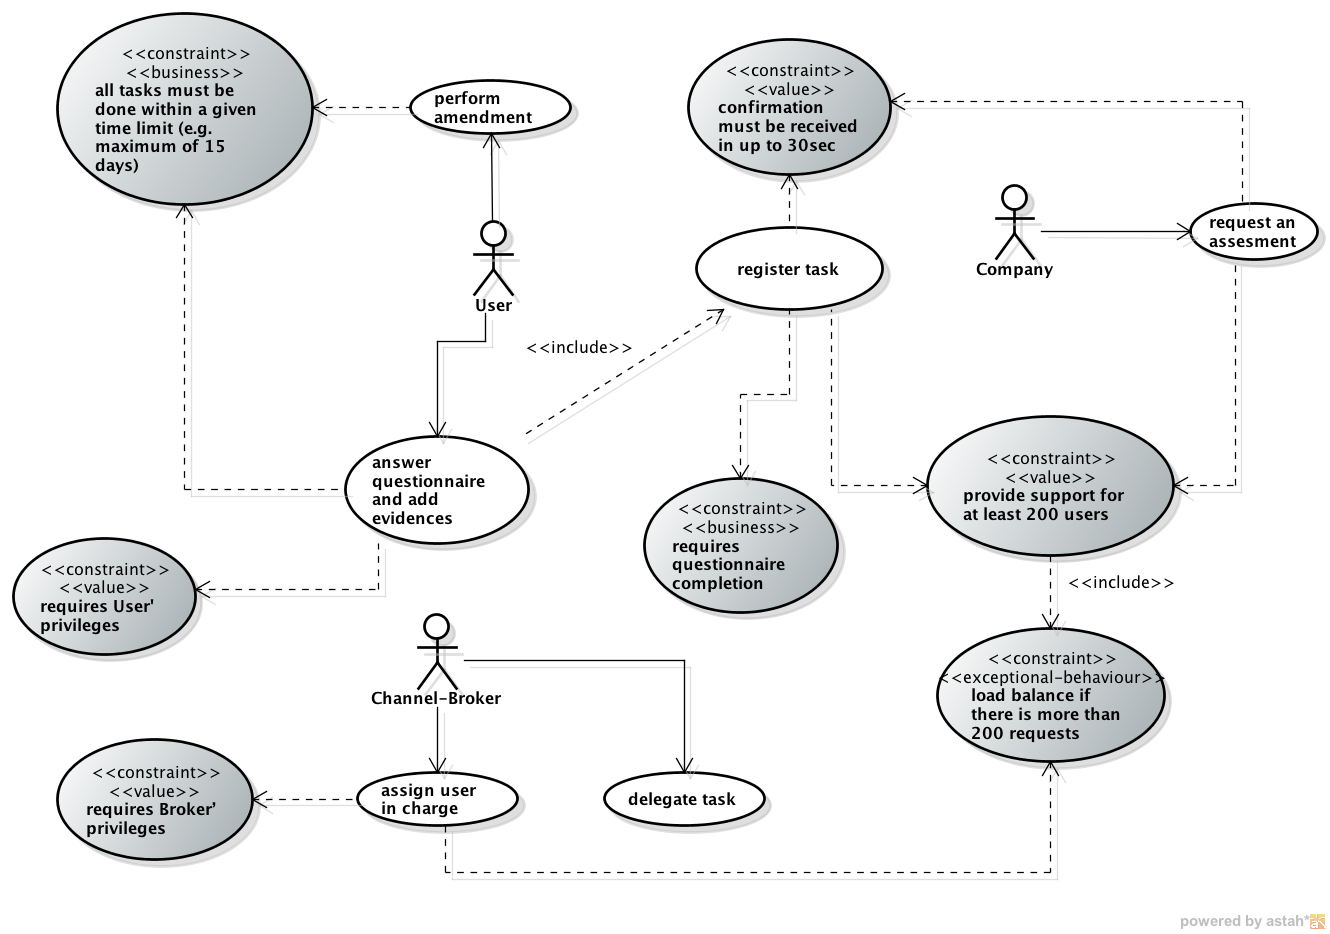
\includegraphics[width=0.9\textwidth]{figs/UseCaseGeneral.png}
\caption{$\pi$-UseCase model for \FlyingPig.\label{fig:piUseCaseModel}}
\end{figure*}


\paragraph{\underline{$\pi$-UseCase Model for \FlyingPig}}~

The $\pi$-UseCase model shown in Figure~\ref{fig:piUseCaseModel} describes the features and constraints for the \FlyingPig\ application.
In this model, three actors are identified: \textit{Company}, \textit{User} and \textit {Broker} represented as stick figures.
In the context of \FlyingPig, Company is the actor requesting a risk evaluation.
A Broker is  responsible for coordinating  the evaluation process, assigning users to be in charge of tasks as well as delegating tasks.
A User, in this model is an actor who answers questionnaires according to the current situation  of the Company.
The User also produces evidence to support facts and performs the necessary amendments to improve the results of the risk assessment.

Each actor is associated to one or more $\pi$-use cases (depicted as white ovals in Fig.~\ref{fig:piUseCaseModel}).
%Use cases
that describe the main functionality of the system.
The $\pi$-UseCase model for \FlyingPig\ defines six $\pi$-use cases.

Each $\pi$-use case may be associated to one or more (non-functional) constraints (coloured ovals in Figure~\ref{fig:piUseCaseModel}).
The mod\-el defines three types of constraints: \textit{value}, \textit{business} or \textit{exceptional behavior}.
Each constraint is identified by the word $<<$\textsf{constraint}$>>$ followed by its type.

%In the case of \FlyingPig, as expressed above the model constraints:
%{\color{red} Anything else here? --M}

\begin{figure*}
\centering
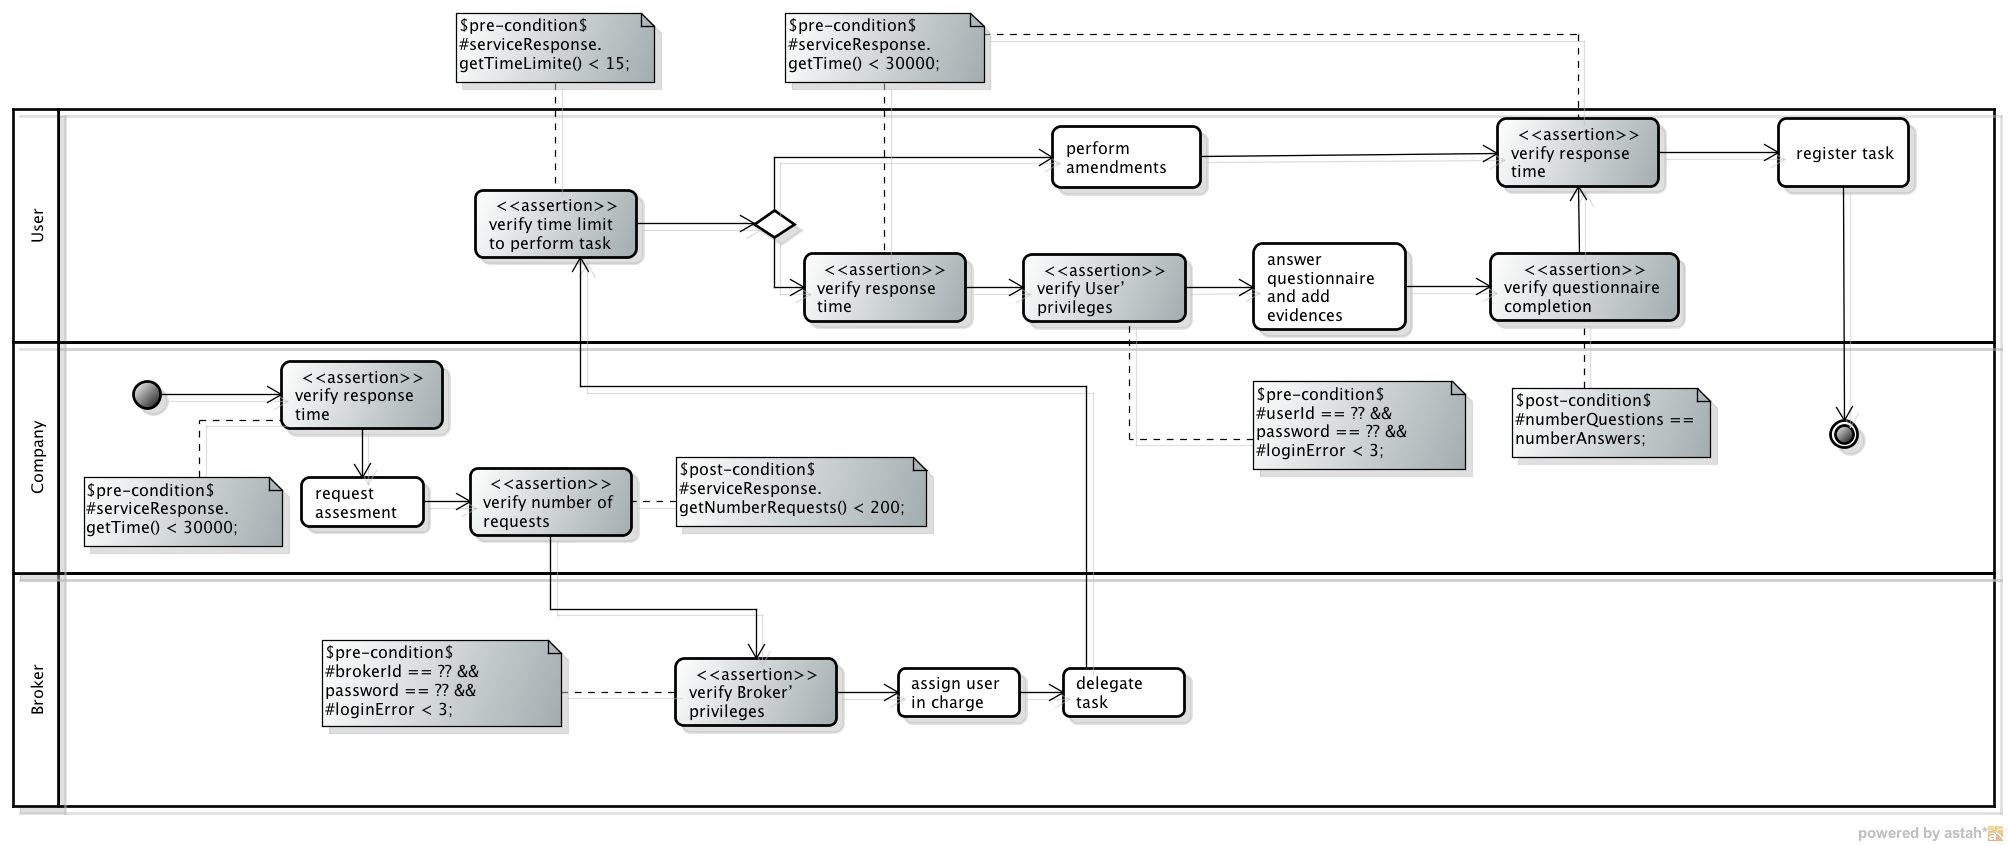
\includegraphics[width=1.0\textwidth]{figs/ServiceProcessGeneralCut.png}
\caption{$\pi$-ServiceProcess model for \FlyingPig.\label{fig:PiServiceProcessModel}}
\end{figure*}

\paragraph{\underline{$\pi$-ServiceProcess Model for \FlyingPig}}~

The $\pi$-ServiceProcess model presents the workflow for \FlyingPig (Figure~\ref{fig:PiServiceProcessModel}).
Actions in this model were obtained by applying the $\pi$-use case transformation rules.
% described in Section~\ref{sec:pewsmetamodel}.

The \textsf{Company}, \textsf{Broker-Channel} and \textsf{User} actors are transformed into lanes that represent the business collaborators.
Use cases are transformed into \textit{actions} and are represented by white boxes.
The restrictions associated to  $\pi$-use cases are transformed into \textit{assertions} (represented by colored boxes) and may be decorated with pre- and post-conditions.
We can see that this model refines the concepts defined in the $\pi$-UseCase model.
The assertions specify those non-functional requirements, as they are seen by the actors.
The next step in the development is to add these assertions to the models that specify the \FlyingPig\ system.

\begin{figure*}
\centering
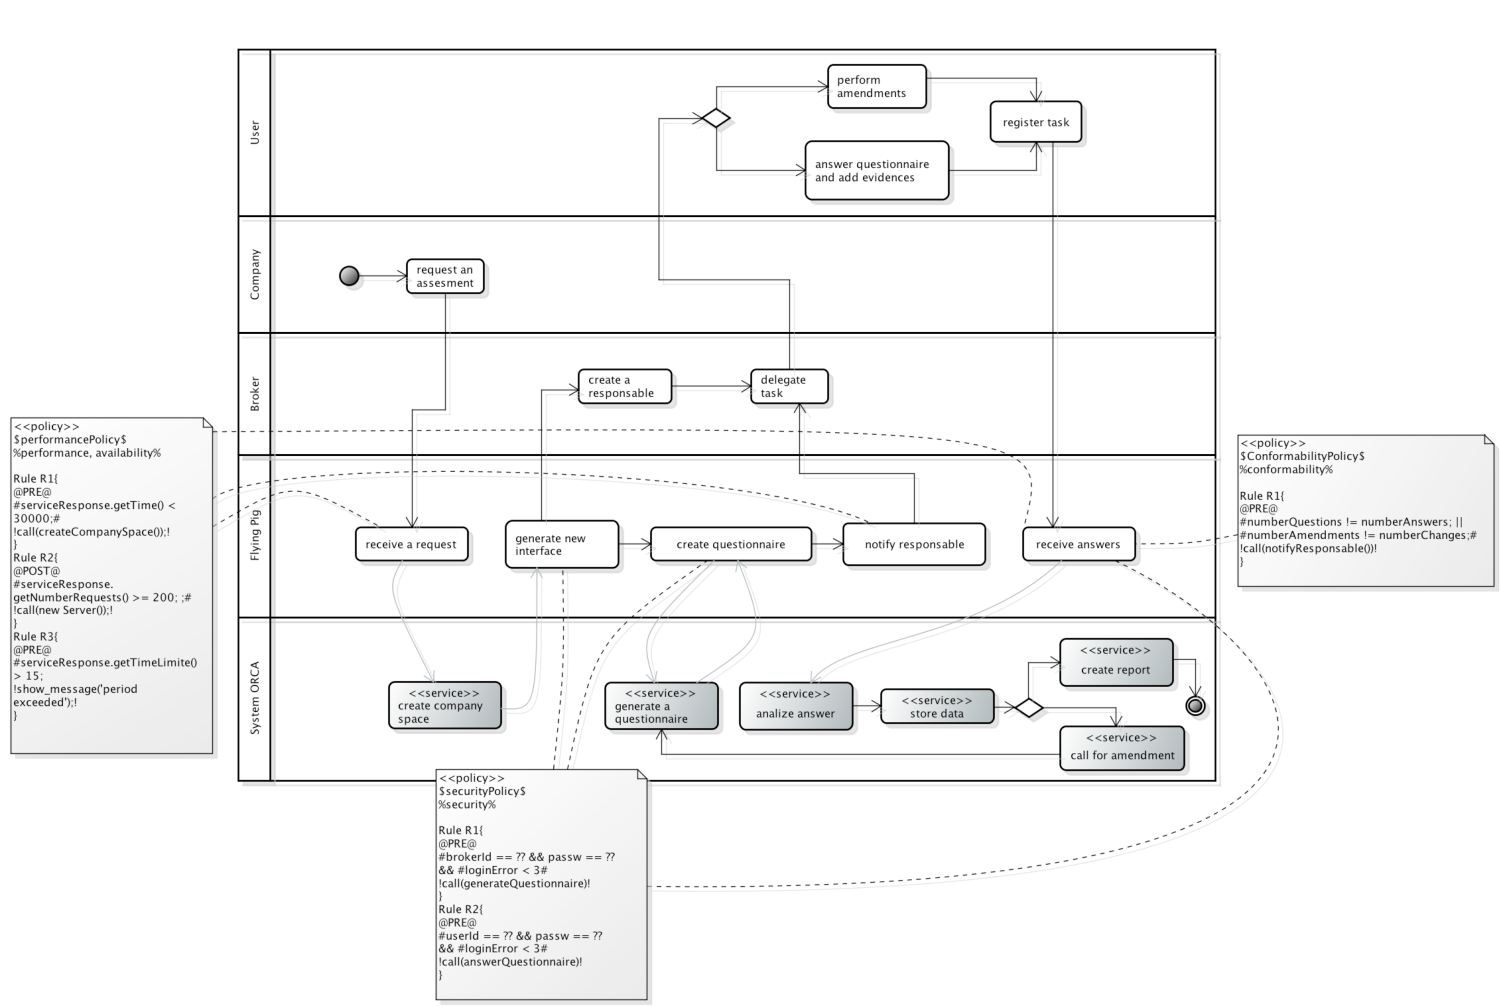
\includegraphics[width=1.0\textwidth]{figs/ServiceCompositionGeneralCut}
\caption{$\pi$-ServiceComposition model for \FlyingPig.\label{fig:PiServiceCompositionModel}}
\end{figure*}

\paragraph{\underline{$\pi$-ServiceComposition Model for \FlyingPig}}~

The model presented in Figure~\ref{fig:PiServiceCompositionModel}
%offers a system-centric view of the application.
%The previous model
is now  completed with the services that provide functions of the application  \FlyingPig\.
The assertions in Figure~\ref{fig:PiServiceProcessModel} are implemented as \textit{policies}.
These policies express the pre- and post-conditions of the previous model.
They are associated to the actions of the system.




%. . - -. . - -. . - -. . - -. . - -. . - -. . - -. . - -. . - -. . - -. . - -. . - -. . - -. . - -. . - -. . - -. . - -. . - -. . - -. . - -. . - -. . - -. . - -. . - -. . - -. . - -
%\subsection{Platform-Specific Model (PSM)}
%. . - -. . - -. . - -. . - -. . - -. . - -. . - -. . - -. . - -. . - -. . - -. . - -. . - -. . - -. . - -. . - -. . - -. . - -. . - -. . - -. . - -. . - -. . - -. . - -. . - -. . - -
\paragraph{\underline{$\pi$-PEWS Model for \FlyingPig}}~

The  PSM model of our case study is obtained by transforming the $\pi$-service composition model into a workflow.
Notice that the workflow for \FlyingPig\ is implemented by using the BPEL constructors~\cite{BPEL}, adding the notion of \textit{policy}.
The model is given in Figure~\ref{fig:piPEWSFlyingPig}.

\begin{figure*}
\begin{verbatim}
//Namespaces specify service URI
namespace orca = www.orca.mx/service.wsdl

//Operations
alias createCompanySpace = portType/createCompanySpace in orca
alias generateQuestionnaire = portType/generateQuestionnaire in orca
alias analizeAnswer = portType/analizeAnswer in orca
alias storeData = portType/storeData in orca
alias createReport = portType/createReport in orca
alias callForAmendments = portType/callForAmendments in orca

//Services
service receiveRequest(R, Id) = createCompanySpace(R, Id)
service generateNewInterface(Id, NULL) = ...
service createQuestionnaire(Id, Q) = generateQuestionnaire(Id, Q)
service notifyResponsable((Id, Q); NULL) = ...
service receiveAnswers((Id, T); P) =
	analizeAnswer((Id, T), NULL) . storeData((Id, T), NULL)
	. ((createReport(Id, P) . return(P)) 
	    + (callForAmendments(Id,T) . return(NULL)))

//Workflow
receiveRequest(R, Id)
||
(generateNewInterface(Id, NULL)
 . createQuestionnaire(Id, Q) . notifyResponsable((Id, Q); NULL))
||
 (receiveAnswers((Id, T); P) . [P != NULL] STOP)*	
\end{verbatim}
\caption{$\pi$-PEWS Model for \FlyingPig}\label{fig:piPEWSFlyingPig}
\end{figure*}



\subsection{Lessons Learned}

Through the example we underlined that every application implements functional aspects that describe its application logic.
Recall that an application logic refers to routines that perform the activities to reach the application objective.
Also there are non functional properties derived from NFR. They refer to strategies to be considered for the application execution like: security, isolation, adaptability, atomicity, and more.
These non functional properties must be ensured at execution time, and they are not completely defined within the application logic.

The challenge is to define them and to associate them with the application logic considering that different to existing solutions that suppose that it is possible to access the execution stat of all the components  of an application and that the application has complete control on them, in the case for service oriented applications  the components are autonomous services
API does not necessarily export information about methods dependency (e.g., in the REST protocol);
they do not share their state (stateless).

Given a set of services with their exported methods, building service-based applications may consist on expressing an application logic as a service composition.
During this task, we must ensure the compliance between the specification and the resulting application.
Software engineering methods (e.g., \cite{2,decastro1,PapazoglouH06}) can help to ensure this compliance, particularly when information systems include several sometimes complex business processes calling Web services or legacy applications exported as services.

As WS-* and similar approaches, our work enables the specification and programming of crosscutting aspects (i.e., atomicity, security, exception handling, persistence).
In contrast to these approaches, our work specifies policies for a services composition in an orthogonal way. Besides, these approaches suppose that non-functional properties are implemented according a the knowledge that a programmer has of a specific application requirements but they are not derived in a methodological way, leading to ad-hoc solutions that can be difficult to reuse. In our approach, once defined the policies for a given application they can be reused and/or specialized for another one with the same requirements or that uses services that impose the same constraints. 